\documentclass[dvipdfmx]{jsarticle}
\setcounter{section}{4}
\setcounter{subsection}{2}
\usepackage{xr}
\externaldocument{2.1.1}
\externaldocument{2.1.2}
\externaldocument{2.1.5}
\externaldocument{2.4.2}
\usepackage{amsmath,amsfonts,amssymb,array,comment,mathtools,url,docmute}
\usepackage{longtable,booktabs,dcolumn,tabularx,mathtools,multirow,colortbl,xcolor}
\usepackage[dvipdfmx]{graphics}
\usepackage{bmpsize}
\usepackage{amsthm}
\usepackage{enumitem}
\setlistdepth{20}
\renewlist{itemize}{itemize}{20}
\setlist[itemize]{label=•}
\renewlist{enumerate}{enumerate}{20}
\setlist[enumerate]{label=\arabic*.}
\setcounter{MaxMatrixCols}{20}
\setcounter{tocdepth}{3}
\newcommand{\rotin}{\text{\rotatebox[origin=c]{90}{$\in $}}}
\renewcommand{\thesection}{第\arabic{section}部}
\renewcommand{\thesubsection}{\arabic{section}.\arabic{subsection}}
\renewcommand{\thesubsubsection}{\arabic{section}.\arabic{subsection}.\arabic{subsubsection}}
\everymath{\displaystyle}
\allowdisplaybreaks[4]
\usepackage{vtable}
\theoremstyle{definition}
\newtheorem{thm}{定理}[subsection]
\newtheorem*{thm*}{定理}
\newtheorem{dfn}{定義}[subsection]
\newtheorem*{dfn*}{定義}
\newtheorem{axs}[dfn]{公理}
\newtheorem*{axs*}{公理}
\renewcommand{\headfont}{\bfseries}
\makeatletter
  \renewcommand{\section}{%
    \@startsection{section}{1}{\z@}%
    {\Cvs}{\Cvs}%
    {\normalfont\huge\headfont\raggedright}}
\makeatother
\makeatletter
  \renewcommand{\subsection}{%
    \@startsection{subsection}{2}{\z@}%
    {0.5\Cvs}{0.5\Cvs}%
    {\normalfont\LARGE\headfont\raggedright}}
\makeatother
\makeatletter
  \renewcommand{\subsubsection}{%
    \@startsection{subsubsection}{3}{\z@}%
    {0.4\Cvs}{0.4\Cvs}%
    {\normalfont\Large\headfont\raggedright}}
\makeatother
\makeatletter
\renewenvironment{proof}[1][\proofname]{\par
  \pushQED{\qed}%
  \normalfont \topsep6\p@\@plus6\p@\relax
  \trivlist
  \item\relax
  {
  #1\@addpunct{.}}\hspace\labelsep\ignorespaces
}{%
  \popQED\endtrivlist\@endpefalse
}
\makeatother
\renewcommand{\proofname}{\textbf{証明}}
\usepackage{tikz,graphics}
\usepackage[dvipdfmx]{hyperref}
\usepackage{pxjahyper}
\hypersetup{
 setpagesize=false,
 bookmarks=true,
 bookmarksdepth=tocdepth,
 bookmarksnumbered=true,
 colorlinks=false,
 pdftitle={},
 pdfsubject={},
 pdfauthor={},
 pdfkeywords={}}
\begin{document}
%\hypertarget{ux53ccux5bfeux6027ux3092ux8868ux3059ux5185ux7a4d}{%
\subsection{双対性を表す内積}%\label{ux53ccux5bfeux6027ux3092ux8868ux3059ux5185ux7a4d}}
%\hypertarget{ux5f62ux5f0fux7684ux306aux53ccux7ddaux5f62ux5f62ux5f0f}{%
\subsubsection{形式的な双線形形式}%\label{ux5f62ux5f0fux7684ux306aux53ccux7ddaux5f62ux5f62ux5f0f}}
\begin{axs}
体$K$上の$m$次元vector空間$V$、$n$次元vector空間$W$が与えられたとき、写像$B:V \times W \rightarrow K$のうち次の性質を満たすものをそのvector空間$V$とそのvector空間$W$との形式的な双線形形式という。
\begin{itemize}
\item
  $\forall k,l \in K\forall\mathbf{u},\mathbf{v} \in V\forall\mathbf{w} \in W$に対し、$B\left( k\mathbf{u} + l\mathbf{v},\mathbf{w} \right) = kB\left( \mathbf{u},\mathbf{w} \right) + lB\left( \mathbf{v},\mathbf{w} \right)$が成り立つ。
\item
  $\forall k,l \in K\forall\mathbf{v} \in V\forall\mathbf{u},\mathbf{w} \in W$に対し、$B\left( \mathbf{v},k\mathbf{u} + l\mathbf{w} \right) = kB\left( \mathbf{v},\mathbf{u} \right) + lB\left( \mathbf{v},\mathbf{w} \right)$が成り立つ。
\end{itemize}
\end{axs}
\begin{dfn}
体$K$上の$n$次元vector空間$V$が与えられたとき、そのvector空間$V$とそのvector空間$V$との形式的な双線形形式$B:V \times V \rightarrow K$のうち次を満たすものを形式的な対称双線形形式という。
\begin{itemize}
\item
  $\forall\mathbf{v},\mathbf{w} \in W$に対し、$B\left( \mathbf{v},\mathbf{w} \right) = B\left( \mathbf{w},\mathbf{v} \right)$が成り立つ。
\end{itemize}
\end{dfn}
\begin{thm}\label{2.4.3.1}
体$K$上の$m$次元vector空間$V$と$n$次元vector空間$W$との形式的な双線形形式$B:V \times W \rightarrow K$が与えられたとき、その体$K$の任意の族々$\left\{ a_{i} \right\}_{i \in \varLambda_{r}}$、$\left\{ b_{i} \right\}_{i \in \varLambda_{s}}$、それらのvector空間たち$V$、$W$の任意の族々$\left\{ \mathbf{v}_{i} \right\}_{i \in \varLambda_{r}}$、$\left\{ \mathbf{w}_{i} \right\}_{i \in \varLambda_{s}}$に対し、次式が成り立つ。
\begin{align*}
B\left( \sum_{i \in \varLambda_{r}} {a_{i}\mathbf{v}_{i}},\sum_{i \in \varLambda_{s}} {b_{i}\mathbf{w}_{i}} \right) = \sum_{(i,j) \in \varLambda_{r} \times \varLambda_{s}} {a_{i}b_{j}B\left( \mathbf{v}_{i},\mathbf{w}_{j} \right)}
\end{align*}
\end{thm}
\begin{proof}
体$K$上の$m$次元vector空間$V$と$n$次元vector空間$W$との形式的な双線形形式$B:V \times W \rightarrow K$が与えられたとき、その体$K$の任意の族々$\left\{ a_{i} \right\}_{i \in \varLambda_{r}}$、$\left\{ b_{i} \right\}_{i \in \varLambda_{s}}$、それらのvector空間たち$V$、$W$の任意の族々$\left\{ \mathbf{v}_{i} \right\}_{i \in \varLambda_{r}}$、$\left\{ \mathbf{w}_{i} \right\}_{i \in \varLambda_{s}}$に対し、数学的帰納法により直ちにわかるように次のようになる。
\begin{align*}
B\left( \sum_{i \in \varLambda_{r}} {a_{i}\mathbf{v}_{i}},\sum_{i \in \varLambda_{s}} {b_{i}\mathbf{w}_{i}} \right) &= \sum_{i \in \varLambda_{r}} {a_{i}B\left( \mathbf{v}_{i},\sum_{j \in \varLambda_{s}} {b_{j}\mathbf{w}_{j}} \right)}\\
&= \sum_{i \in \varLambda_{r}} {\sum_{j \in \varLambda_{s}} {a_{i}b_{j}B\left( \mathbf{v}_{i},\mathbf{w}_{j} \right)}}\\
&= \sum_{(i,j) \in \varLambda_{r} \times \varLambda_{s}} {a_{i}b_{j}B\left( \mathbf{v}_{i},\mathbf{w}_{j} \right)}
\end{align*}
\end{proof}
\begin{thm}\label{2.4.3.2}
体$K$上の$m$次元vector空間$V$と$n$次元vector空間$W$との形式的な双線形形式たち$B:V \times W \rightarrow K$、$C:V \times W \rightarrow K$が与えられたとき、$\forall a,b \in K$に対し、写像$aB + bC:V \times W \rightarrow K$もそれらのvector空間たち$V$、$W$との形式的な双線形形式である。
\end{thm}
\begin{proof}
体$K$上の$m$次元vector空間$V$と$n$次元vector空間$W$との形式的な双線形形式たち$B:V \times W \rightarrow K$、$C:V \times W \rightarrow K$が与えられたとき、$\forall a,b \in K$に対し、写像$aB + bC:V \times W \rightarrow K$について、$\forall k,l \in K\forall\mathbf{u},\mathbf{v} \in V\forall\mathbf{w} \in W$に対し、次のようになる。
\begin{align*}
(aB + bC)\left( k\mathbf{u} + l\mathbf{v},\mathbf{w} \right) &= aB\left( k\mathbf{u} + l\mathbf{v},\mathbf{w} \right) + bC\left( k\mathbf{u} + l\mathbf{v},\mathbf{w} \right)\\
&= a\left( kB\left( \mathbf{u},\mathbf{w} \right) + lB\left( \mathbf{v},\mathbf{w} \right) \right) + b\left( kC\left( \mathbf{u},\mathbf{w} \right) + lC\left( \mathbf{v},\mathbf{w} \right) \right)\\
&= akB\left( \mathbf{u},\mathbf{w} \right) + alB\left( \mathbf{v},\mathbf{w} \right) + bkC\left( \mathbf{u},\mathbf{w} \right) + blC\left( \mathbf{v},\mathbf{w} \right)\\
&= k\left( aB\left( \mathbf{u},\mathbf{w} \right) + bC\left( \mathbf{u},\mathbf{w} \right) \right) + l\left( aB\left( \mathbf{v},\mathbf{w} \right) + bC\left( \mathbf{v},\mathbf{w} \right) \right)\\
&= k(aB + bC)\left( \mathbf{u},\mathbf{w} \right) + l(aB + bC)\left( \mathbf{v},\mathbf{w} \right)
\end{align*}
また、$\forall k,l \in K\forall\mathbf{v} \in V\forall\mathbf{u},\mathbf{w} \in W$に対し、次のようになる。
\begin{align*}
(aB + bC)\left( \mathbf{u},k\mathbf{v} + l\mathbf{w} \right) &= aB\left( \mathbf{u},k\mathbf{v} + l\mathbf{w} \right) + bC\left( \mathbf{u},k\mathbf{v} + l\mathbf{w} \right)\\
&= a\left( kB\left( \mathbf{u},\mathbf{v} \right) + lB\left( \mathbf{u},\mathbf{w} \right) \right) + b\left( kC\left( \mathbf{u},\mathbf{v} \right) + lC\left( \mathbf{u},\mathbf{w} \right) \right)\\
&= akB\left( \mathbf{u},\mathbf{v} \right) + alB\left( \mathbf{u},\mathbf{w} \right) + bkC\left( \mathbf{u},\mathbf{v} \right) + blC\left( \mathbf{u},\mathbf{w} \right)\\
&= k\left( aB\left( \mathbf{u},\mathbf{v} \right) + bC\left( \mathbf{u},\mathbf{v} \right) \right) + l\left( aB\left( \mathbf{u},\mathbf{w} \right) + bC\left( \mathbf{u},\mathbf{w} \right) \right)\\
&= k(aB + bC)\left( \mathbf{u},\mathbf{v} \right) + l(aB + bC)\left( \mathbf{u},\mathbf{w} \right)
\end{align*}
よって、その写像$kB + lC:V \times V \rightarrow K$もそれらのvector空間たち$V$、$W$との形式的な双線形形式である。
\end{proof}
\begin{dfn}
体$K$上の$m$次元vector空間$V$と$n$次元vector空間$W$との形式的な双線形形式$B:V \times W \rightarrow K$が与えられたとき、それらのvector空間たち$V$、$W$の$\alpha = \left\langle \mathbf{v}_{i} \right\rangle_{i \in \varLambda_{m}}$、$\beta = \left\langle \mathbf{w}_{i} \right\rangle_{i \in \varLambda_{n}}$なる基底たちそれぞれ$\alpha$、$\beta$がとられれば、次式のように定義されるその集合$M_{mn}(K)$における行列$A_{mn}$をその双線形形式$B$のその基底の組$(\alpha,\beta)$に関する表現行列、表現などといい、
\begin{align*}
A_{nn} = \left( B\left( \mathbf{v}_{i},\mathbf{w}_{j} \right) \right)_{(i,j) \in \varLambda_{m} \times \varLambda_{n}}
\end{align*}
以下、その行列$A_{nn}$を$[ B]_{(\alpha,\beta)}$とかく。
\end{dfn}
\begin{thm}\label{2.4.3.3}
体$K$上の$m$次元vector空間$V$と$n$次元vector空間$W$との形式的な双線形形式$B:V \times W \rightarrow K$が与えられたとき、それらのvector空間たち$V$、$W$の$\alpha = \left\langle \mathbf{v}_{i} \right\rangle_{i \in \varLambda_{m}}$、$\beta = \left\langle \mathbf{w}_{i} \right\rangle_{i \in \varLambda_{n}}$なる基底たちそれぞれ$\alpha$、$\beta$がとられ、さらに、その双線形形式$B$のその基底の組$(\alpha,\beta)$に関する表現行列$[ B]_{(\alpha,\beta)}$が$[ B]_{(\alpha,\beta)} = \left( B_{ij} \right)_{(i,j) \in \varLambda_{m} \times \varLambda_{n}}$と成分表示されれば、$\forall\mathbf{v},\mathbf{w} \in V$に対し、その体$K$の族々$\left\{ a_{i} \right\}_{i \in \varLambda_{m}}$、$\left\{ b_{i} \right\}_{i \in \varLambda_{n}}$を用いて次のようにおくと、
\begin{align*}
\mathbf{v} = \sum_{i \in \varLambda_{m}} {a_{i}\mathbf{v}_{i}},\ \ \mathbf{w} = \sum_{i \in \varLambda_{n}} {b_{i}\mathbf{v}_{i}}
\end{align*}
それらの基底たち$\alpha$、$\beta$に関する基底変換における線形同型写像たち$\varphi_{\alpha}$、$\varphi_{\beta}$を用いれば、次式が成り立つ。
\begin{align*}
B\left( \mathbf{v},\mathbf{w} \right) = \sum_{(i,j) \in \varLambda_{m} \times \varLambda_{n}} {a_{i}b_{j}B_{ij}} ={}^{t}\varphi_{\alpha}^{- 1}\left( \mathbf{v} \right)[ B]_{(\alpha,\beta)}\varphi_{\beta}^{- 1}\left( \mathbf{w} \right)
\end{align*}
\end{thm}
\begin{proof}
体$K$上の$m$次元vector空間$V$と$n$次元vector空間$W$との形式的な双線形形式$B:V \times W \rightarrow K$が与えられたとき、それらのvector空間たち$V$、$W$の$\alpha = \left\langle \mathbf{v}_{i} \right\rangle_{i \in \varLambda_{m}}$、$\beta = \left\langle \mathbf{w}_{i} \right\rangle_{i \in \varLambda_{n}}$なる基底たちそれぞれ$\alpha$、$\beta$がとられ、さらに、その双線形形式$B$のその基底の組$(\alpha,\beta)$に関する表現行列$[ B]_{(\alpha,\beta)}$が$[ B]_{(\alpha,\beta)} = \left( B_{ij} \right)_{(i,j) \in \varLambda_{m} \times \varLambda_{n}}$と成分表示されれば、$\forall\mathbf{v},\mathbf{w} \in V$に対し、その体$K$の族々$\left\{ a_{i} \right\}_{i \in \varLambda_{m}}$、$\left\{ b_{i} \right\}_{i \in \varLambda_{n}}$を用いて次のようにおくと、
\begin{align*}
\mathbf{v} = \sum_{i \in \varLambda_{m}} {a_{i}\mathbf{v}_{i}},\ \ \mathbf{w} = \sum_{i \in \varLambda_{n}} {b_{i}\mathbf{v}_{i}}
\end{align*}
定理\ref{2.4.3.1}より次のようになる。
\begin{align*}
B\left( \mathbf{v},\mathbf{w} \right) = B\left( \sum_{i \in \varLambda_{m}} {a_{i}\mathbf{v}_{i}},\sum_{i \in \varLambda_{n}} {b_{i}\mathbf{v}_{i}} \right) = \sum_{(i,j) \in \varLambda_{m} \times \varLambda_{n}} {a_{i}b_{j}B\left( \mathbf{v}_{i},\mathbf{v}_{j} \right)}
\end{align*}
そこで、双線形形式の表現行列の定義より$B\left( \mathbf{v}_{i},\mathbf{v}_{j} \right) = B_{ij}$が成り立つので、次のようになる。
\begin{align*}
B\left( \mathbf{v},\mathbf{w} \right) = \sum_{(i,j) \in \varLambda_{m} \times \varLambda_{n}} {a_{i}b_{j}B_{ij}}
\end{align*}\par
また、それらの基底たち$\alpha$、$\beta$に関する基底変換における線形同型写像たち$\varphi_{\alpha}$、$\varphi_{\beta}$を用いれば、次のようになるので、
\begin{align*}
\varphi_{\alpha}^{- 1}\left( \mathbf{v} \right) = \begin{pmatrix}
a_{1} \\
a_{2} \\
 \vdots \\
a_{m} \\
\end{pmatrix},\ \ \varphi_{\beta}^{- 1}\left( \mathbf{w} \right) = \begin{pmatrix}
b_{1} \\
b_{2} \\
 \vdots \\
b_{n} \\
\end{pmatrix}
\end{align*}
したがって、次のようになる。
\begin{align*}
{}^{t}\varphi_{\alpha}^{- 1}\left( \mathbf{v} \right)[ B]_{(\alpha,\beta)}\varphi_{\beta}^{- 1}\left( \mathbf{w} \right) &={}^{t}\begin{pmatrix}
a_{1} \\
a_{2} \\
 \vdots \\
a_{m} \\
\end{pmatrix}\begin{pmatrix}
B_{11} & B_{12} & \cdots & B_{1n} \\
B_{21} & B_{22} & \cdots & B_{2n} \\
 \vdots & \vdots & \ddots & \vdots \\
B_{m1} & B_{m2} & \cdots & B_{mn} \\
\end{pmatrix}\begin{pmatrix}
b_{1} \\
b_{2} \\
 \vdots \\
b_{n} \\
\end{pmatrix}\\
&= \begin{pmatrix}
a_{1} & a_{2} & \cdots & a_{m} \\
\end{pmatrix}\begin{pmatrix}
B_{11} & B_{12} & \cdots & B_{1n} \\
B_{21} & B_{22} & \cdots & B_{2n} \\
 \vdots & \vdots & \ddots & \vdots \\
B_{m1} & B_{m2} & \cdots & B_{mn} \\
\end{pmatrix}\begin{pmatrix}
b_{1} \\
b_{2} \\
 \vdots \\
b_{n} \\
\end{pmatrix}\\
&= \begin{pmatrix}
a_{1} & a_{2} & \cdots & a_{m} \\
\end{pmatrix}\begin{pmatrix}
\sum_{j \in \varLambda_{n}} {b_{j}B_{1j}} \\
\sum_{j \in \varLambda_{n}} {b_{j}B_{2j}} \\
 \vdots \\
\sum_{j \in \varLambda_{n}} {b_{j}B_{mj}} \\
\end{pmatrix}\\
&= \sum_{i \in \varLambda_{m}} {\sum_{j \in \varLambda_{n}} {a_{i}b_{j}B_{ij}}} = \sum_{(i,j) \in \varLambda_{m} \times \varLambda_{n}} {a_{i}b_{j}B_{ij}}
\end{align*}
よって、次式が成り立つ。
\begin{align*}
B\left( \mathbf{v},\mathbf{w} \right) = \sum_{(i,j) \in \varLambda_{m} \times \varLambda_{n}} {a_{i}b_{j}B_{ij}} ={}^{t}\varphi_{\alpha}^{- 1}\left( \mathbf{v} \right)[ B]_{(\alpha,\beta)}\varphi_{\beta}^{- 1}\left( \mathbf{w} \right)
\end{align*}
\end{proof}
\begin{thm}\label{2.4.3.4}
体$K$上の$m$次元vector空間$V$と$n$次元vector空間$W$との形式的な双線形形式$B:V \times W \rightarrow K$が与えられたとき、それらのvector空間たち$V$、$W$の$\alpha = \left\langle \mathbf{v}_{i} \right\rangle_{i \in \varLambda_{m}}$、$\beta = \left\langle \mathbf{w}_{i} \right\rangle_{i \in \varLambda_{n}}$なる基底たちそれぞれ$\alpha$、$\beta$がとられて、$\forall A_{mn} \in M_{mn}(K)$に対し、それらの基底たち$\alpha$、$\beta$に関する基底変換における線形同型写像たち$\varphi_{\alpha}$、$\varphi_{\beta}$を用いて次式のような写像$B_{A_{mn}}$を考えよう。
\begin{align*}
B_{A_{mn}}:V \times W \rightarrow K;\left( \mathbf{v},\mathbf{w} \right) \mapsto{}^{t}\varphi_{\alpha}^{- 1}\left( \mathbf{v} \right)A_{mn}\varphi_{\beta}^{- 1}\left( \mathbf{w} \right)
\end{align*}
このとき、次のことが成り立つ。
\begin{itemize}
\item
  その写像$B_{A_{mn}}$はそれらのvector空間たち$V$、$W$との形式的な双線形形式である。
\item
  $A_{mn} = \left( a_{ij} \right)_{(i,j) \in \varLambda_{m} \times \varLambda_{n}}$とおかれれば、$\forall i \in \varLambda_{m}\forall j \in \varLambda_{n}$に対し、$B_{A_{mn}}\left( \mathbf{v}_{i},\mathbf{v}_{j} \right) = a_{ij}$が成り立つ。
\item
  $\left[ B_{A_{mn}} \right]_{(\alpha,\beta)} = A_{mn}$が成り立つ。
\end{itemize}
\end{thm}
\begin{proof}
体$K$上の$m$次元vector空間$V$と$n$次元vector空間$W$との形式的な双線形形式$B:V \times W \rightarrow K$が与えられたとき、それらのvector空間たち$V$、$W$の$\alpha = \left\langle \mathbf{v}_{i} \right\rangle_{i \in \varLambda_{m}}$、$\beta = \left\langle \mathbf{w}_{i} \right\rangle_{i \in \varLambda_{n}}$なる基底たちそれぞれ$\alpha$、$\beta$がとられて、$\forall A_{mn} \in M_{mn}(K)$に対し、それらの基底たち$\alpha$、$\beta$に関する基底変換における線形同型写像たち$\varphi_{\alpha}$、$\varphi_{\beta}$を用いて次式のような写像$B_{A_{mn}}$を考えよう。
\begin{align*}
B_{A_{mn}}:V \times W \rightarrow K;\left( \mathbf{v},\mathbf{w} \right) \mapsto{}^{t}\varphi_{\alpha}^{- 1}\left( \mathbf{v} \right)A_{mn}\varphi_{\beta}^{- 1}\left( \mathbf{w} \right)
\end{align*}
このとき、$\forall k,l \in K\forall\mathbf{u},\mathbf{v} \in V\forall\mathbf{w} \in W$に対し、次のようになる。
\begin{align*}
B_{A_{mn}}\left( k\mathbf{u} + l\mathbf{v},\mathbf{w} \right) &={}^{t}\varphi_{\alpha}^{- 1}\left( k\mathbf{u} + l\mathbf{v} \right)A_{mn}\varphi_{\beta}^{- 1}\left( \mathbf{w} \right)\\
&= \left( k{}^{t}\varphi_{\alpha}^{- 1}\left( \mathbf{u} \right) + l{}^{t}\varphi_{\alpha}^{- 1}\left( \mathbf{v} \right) \right)A_{mn}\varphi_{\beta}^{- 1}\left( \mathbf{w} \right)\\
&= k{}^{t}\varphi_{\alpha}^{- 1}\left( \mathbf{u} \right)A_{mn}\varphi_{\beta}^{- 1}\left( \mathbf{w} \right) + l{}^{t}\varphi_{\alpha}^{- 1}\left( \mathbf{v} \right)A_{mn}\varphi_{\beta}^{- 1}\left( \mathbf{w} \right)\\
&= kB_{A_{mn}}\left( \mathbf{u},\mathbf{w} \right) + lB_{A_{mn}}\left( \mathbf{v},\mathbf{w} \right)
\end{align*}
また、$\forall k,l \in K\forall\mathbf{v} \in V\forall\mathbf{u},\mathbf{w} \in W$に対し、次のようになる。
\begin{align*}
B_{A_{mn}}\left( \mathbf{v},k\mathbf{u} + l\mathbf{w} \right) &={}^{t}\varphi_{\alpha}^{- 1}\left( \mathbf{v} \right)A_{mn}\varphi_{\beta}^{- 1}\left( k\mathbf{u} + l\mathbf{w} \right)\\
&={}^{t}\varphi_{\alpha}^{- 1}\left( \mathbf{v} \right)A_{mn}\left( k\varphi_{\beta}^{- 1}\left( \mathbf{u} \right) + l\varphi_{\beta}^{- 1}\left( \mathbf{w} \right) \right)\\
&= k{}^{t}\varphi_{\alpha}^{- 1}\left( \mathbf{v} \right)A_{mn}\varphi_{\beta}^{- 1}\left( \mathbf{u} \right) + l{}^{t}\varphi_{\alpha}^{- 1}\left( \mathbf{v} \right)A_{mn}\varphi_{\beta}^{- 1}\left( \mathbf{w} \right)\\
&= kB_{A_{mn}}\left( \mathbf{v},\mathbf{u} \right) + lB_{A_{mn}}\left( \mathbf{v},\mathbf{w} \right)
\end{align*}
よって、その写像$B_{A_{mn}}$はそのvector空間$V$上の双線形形式である。\par
$A_{mn} = \left( a_{ij} \right)_{(i,j) \in \varLambda_{m} \times \varLambda_{n}}$とおかれれば、$\forall i \in \varLambda_{m}\forall j \in \varLambda_{n}$に対し、vector空間$K^{m}$、$K^{n}$の標準基底のうち第$i'$成分が$1$でこれ以外の成分が$0$であるようなvectors$\mathbf{d}_{i'}$、$\mathbf{e}_{i'}$を用いて次のようになる。
\begin{align*}
B_{A_{mn}}\left( \mathbf{v}_{i},\mathbf{v}_{j} \right) &={}^{t}\varphi_{\alpha}^{- 1}\left( \mathbf{v}_{i} \right)A_{mn}\varphi_{\beta}^{- 1}\left( \mathbf{v}_{j} \right)\\
&={}^{t}\mathbf{d}_{i}A_{mn}\mathbf{e}_{j}\\
&= \begin{pmatrix}
0 & \cdots & 1 & \cdots & 0 \\
\end{pmatrix}\begin{pmatrix}
a_{11} & \cdots & a_{1j} & \cdots & a_{1n} \\
 \vdots & \ddots & \vdots & \ddots & \vdots \\
a_{i1} & \cdots & a_{ij} & \cdots & a_{in} \\
 \vdots & \ddots & \vdots & \ddots & \vdots \\
a_{m1} & \cdots & a_{mj} & \cdots & a_{mn} \\
\end{pmatrix}\begin{pmatrix}
0 \\
 \vdots \\
1 \\
 \vdots \\
0 \\
\end{pmatrix}\\
&= \begin{pmatrix}
0 & \cdots & 1 & \cdots & 0 \\
\end{pmatrix}\begin{pmatrix}
a_{1j} \\
 \vdots \\
a_{ij} \\
 \vdots \\
a_{mj} \\
\end{pmatrix} = a_{ij}
\end{align*}\par
あとは、表現行列の定義より明らかに$\left[ B_{A_{mn}} \right]_{(\alpha,\beta)} = A_{mn}$が成り立つ。
\end{proof}
\begin{thm}\label{2.4.3.5}
体$K$上の$n$次元vector空間$V$が与えられたとき、そのvector空間$V$とそのvector空間$V$との形式的な双線形形式$B:V \times V \rightarrow K$が与えられたとき、$\alpha = \left\langle \mathbf{v}_{i} \right\rangle_{i \in \varLambda_{n}}$なるそのvector空間$V$の基底$\alpha$がとられれば、その形式的な双線形形式$B$が形式的な対称双線形形式となるならそのときに限り、その双線形形式$B$のその基底の組$(\alpha,\alpha)$に関する表現行列$[ B]_{(\alpha,\alpha)}$が対称行列となる、即ち、$[ B]_{(\alpha,\alpha)} ={}^{t}[ B]_{(\alpha,\alpha)}$が成り立つ。
\end{thm}
\begin{proof}
体$K$上の$n$次元vector空間$V$が与えられたとき、そのvector空間$V$とそのvector空間$V$との形式的な双線形形式$B:V \times V \rightarrow K$が与えられたとき、$\alpha = \left\langle \mathbf{v}_{i} \right\rangle_{i \in \varLambda_{n}}$なるそのvector空間$V$の基底$\alpha$がとられれば、その形式的な双線形形式$B$が形式的な対称双線形形式となるなら、$\forall i,j \in \varLambda_{n}$に対し、$B\left( \mathbf{v}_{i},\mathbf{v}_{j} \right) = B\left( \mathbf{v}_{j},\mathbf{v}_{i} \right)$が成り立つ。ここで、$[ B]_{(\alpha,\alpha)} = \left( B_{ij} \right)_{(i,j) \in \varLambda_{n}^{2}}$と成分表示されれば、次のようになるので、
\begin{align*}
B_{ij} = B\left( \mathbf{v}_{i},\mathbf{v}_{j} \right) = B\left( \mathbf{v}_{j},\mathbf{v}_{i} \right) = B_{ji}
\end{align*}
次のようになる。
\begin{align*}
[ B]_{(\alpha,\alpha)} = \left( B_{ij} \right)_{(i,j) \in \varLambda_{n}^{2}} = \left( B_{ji} \right)_{(i,j) \in \varLambda_{n}^{2}} ={}^{t}\left( B_{ij} \right)_{(i,j) \in \varLambda_{n}^{2}} ={}^{t}[ B]_{(\alpha,\alpha)}
\end{align*}\par
逆に、その双線形形式$B$のその基底の組$(\alpha,\alpha)$に関する表現行列$[ B]_{(\alpha,\alpha)}$が対称行列となる、即ち、$[ B]_{(\alpha,\alpha)} ={}^{t}[ B]_{(\alpha,\alpha)}$が成り立つなら、その基底$\alpha$に関する基底変換における線形同型写像$\varphi_{\alpha}$を用いて、$\forall\mathbf{v},\mathbf{w} \in V$に対し、定理\ref{2.4.3.3}より次のようになる。
\begin{align*}
B\left( \mathbf{v},\mathbf{w} \right) &={}^{t}\varphi_{\alpha}^{- 1}\left( \mathbf{v} \right)[ B]_{(\alpha,\alpha)}\varphi_{\alpha}^{- 1}\left( \mathbf{w} \right)\\
&={}^{t}\varphi_{\alpha}^{- 1}\left( \mathbf{v} \right){}^{t}{}^{t}[ B]_{(\alpha,\alpha)}{}^{t}{}^{t}\varphi_{\alpha}^{- 1}\left( \mathbf{w} \right)\\
&={}^{t}\left({}^{t}\varphi_{\alpha}^{- 1}\left( \mathbf{w} \right){}^{t}[ B]_{(\alpha,\alpha)}\varphi_{\alpha}^{- 1}\left( \mathbf{v} \right) \right)\\
&={}^{t}\left({}^{t}\varphi_{\alpha}^{- 1}\left( \mathbf{w} \right)[ B]_{(\alpha,\alpha)}\varphi_{\alpha}^{- 1}\left( \mathbf{v} \right) \right)\\
&={}^{t}B\left( \mathbf{w},\mathbf{v} \right) = B\left( \mathbf{w},\mathbf{v} \right)
\end{align*}
\end{proof}
%\hypertarget{ux975eux9000ux5316ux306aux53ccux7ddaux5f62ux5f62ux5f0f}{%
\subsubsection{非退化な双線形形式}%\label{ux975eux9000ux5316ux306aux53ccux7ddaux5f62ux5f62ux5f0f}}
\begin{dfn}
体$K$上の$m$次元vector空間$V$と$n$次元vector空間$W$との形式的な双線形形式$B:V \times W \rightarrow K$が与えられたとき、これが次のことを満たすとき、その双線形形式$B$は非退化であるという\footnote{論理式に直すと、$\forall\mathbf{v} \in V\left[ B\left( \mathbf{v},\mathbf{w} \right) = 0 \right] \Rightarrow \mathbf{w} = \mathbf{0}$となっていることに注意されたい。}。
\begin{itemize}
\item
  $\forall\mathbf{v} \in V$に対し、$B\left( \mathbf{v},\mathbf{w} \right) = 0$が成り立つなら、$\mathbf{w} = \mathbf{0}$が成り立つ。
\item
  $\forall\mathbf{w} \in W$に対し、$B\left( \mathbf{v},\mathbf{w} \right) = 0$が成り立つなら、$\mathbf{v} = 0$が成り立つ。
\end{itemize}
\end{dfn}
\begin{dfn}
体$K$上の$m$次元vector空間$V$と$n$次元vector空間$W$との形式的な双線形形式$B:V \times W \rightarrow K$が与えられたとき、これから$\mathbf{v} \in V$、$\mathbf{w} \in W$を用いて次式のように定義される線形写像$\varPhi_{B,l}\left( \mathbf{w} \right)$、$\varPhi_{B,r}\left( \mathbf{v} \right)$を、ここでは、それぞれそのvector空間$V$上のその形式的な双線形形式$B$からそのvector$\mathbf{w}$によって誘導される左の線形形式、そのvector空間$W$上のその形式的な双線形形式$B$からそのvector$\mathbf{v}$によって誘導される右の線形形式ということにする。
\begin{align*}
\varPhi_{B,l}\left( \mathbf{w} \right)&:V \rightarrow K;\mathbf{v} \mapsto B\left( \mathbf{v},\mathbf{w} \right)\\
\varPhi_{B,r}\left( \mathbf{v} \right)&:V \rightarrow K;\mathbf{w} \mapsto B\left( \mathbf{v},\mathbf{w} \right)
\end{align*}
\end{dfn}
\begin{thm}\label{2.4.3.6}
体$K$上の$m$次元vector空間$V$と$n$次元vector空間$W$との形式的な双線形形式$B:V \times W \rightarrow K$が与えられたとき、$\forall\mathbf{v} \in V\forall\mathbf{w} \in W$に対し、そのvector空間$V$上のその形式的な双線形形式$B$からそのvector$\mathbf{w}$によって誘導される左の線形形式$\varPhi_{B,l}\left( \mathbf{w} \right)$、そのvector空間$W$上のその形式的な双線形形式$B$からそのvector$\mathbf{v}$によって誘導される右の線形形式$\varPhi_{B,r}\left( \mathbf{v} \right)$はいずれも線形写像である。これゆえに、$\forall\mathbf{v} \in V\forall\mathbf{w} \in W$に対し、$\varPhi_{B,l}\left( \mathbf{w} \right) \in V^{*}$かつ$\varPhi_{B,r}\left( \mathbf{v} \right) \in W^{*}$が成り立ちこのような呼び方でも混乱は生じなかろう。
\end{thm}
\begin{proof}
体$K$上の$m$次元vector空間$V$と$n$次元vector空間$W$との形式的な双線形形式$B:V \times W \rightarrow K$が与えられたとき、$\forall\mathbf{w} \in W$に対し、そのvector空間$V$上のその形式的な双線形形式$B$からそのvector$\mathbf{w}$によって誘導される左の線形形式$\varPhi_{B,l}\left( \mathbf{w} \right)$について、$\forall k,l \in K\forall\mathbf{u},\mathbf{v} \in V$に対し、次のようになる。
\begin{align*}
\varPhi_{B,l}\left( \mathbf{w} \right)\left( k\mathbf{u} + l\mathbf{v} \right) &= B\left( k\mathbf{u} + l\mathbf{v},\mathbf{w} \right)\\
&= kB\left( \mathbf{u},\mathbf{w} \right) + lB\left( \mathbf{v},\mathbf{w} \right)\\
&= k\varPhi_{B,l}\left( \mathbf{w} \right)\left( \mathbf{u} \right) + l\varPhi_{B,l}\left( \mathbf{w} \right)\left( \mathbf{v} \right)
\end{align*}\par
同様に、$\forall\mathbf{v} \in V$に対し、そのvector空間$W$上のその形式的な双線形形式$B$からそのvector$\mathbf{v}$によって誘導される右の線形形式$\varPhi_{B,r}\left( \mathbf{v} \right)$について、$\forall k,l \in K\forall\mathbf{u},\mathbf{w} \in W$に対し、次のようになる。
\begin{align*}
\varPhi_{B,r}\left( \mathbf{v} \right)\left( k\mathbf{u} + l\mathbf{w} \right) &= B\left( \mathbf{v},k\mathbf{u} + l\mathbf{w} \right)\\
&= kB\left( \mathbf{v},\mathbf{u} \right) + lB\left( \mathbf{v},\mathbf{w} \right)\\
&= k\varPhi_{B,r}\left( \mathbf{v} \right)\left( \mathbf{u} \right) + l\varPhi_{B,r}\left( \mathbf{v} \right)\left( \mathbf{w} \right)
\end{align*}
\end{proof}
\begin{dfn}
体$K$上の$m$次元vector空間$V$と$n$次元vector空間$W$との形式的な双線形形式$B:V \times W \rightarrow K$が与えられたとき、そのvector空間$V$上のその形式的な双線形形式$B$からそのvector$\mathbf{w}$によって誘導される左の線形形式$\varPhi_{B,l}\left( \mathbf{w} \right)$、そのvector空間$W$上のその形式的な双線形形式$B$からそのvector$\mathbf{v}$によって誘導される右の線形形式$\varPhi_{B,r}\left( \mathbf{v} \right)$を用いた次式のように定義される写像たち$\varPhi_{B,l}$、$\varPhi_{B,r}$をそれぞれその形式的な双線形形式$B$から左の線形形式に誘導する線形写像、その形式的な双線形形式$B$から右の線形形式に誘導する線形写像ということにする。
\begin{align*}
\varPhi_{B,l}&:W \rightarrow V^{*};\mathbf{w} \mapsto \left( \varPhi_{B,l}\left( \mathbf{w} \right):V \rightarrow K;\mathbf{v} \mapsto B\left( \mathbf{v},\mathbf{w} \right) \right)\\
\varPhi_{B,r}&:V \rightarrow W^{*};\mathbf{v} \mapsto \left( \varPhi_{B,r}\left( \mathbf{v} \right):W \rightarrow K;\mathbf{w} \mapsto B\left( \mathbf{v},\mathbf{w} \right) \right)
\end{align*}
\end{dfn}
\begin{thm}\label{2.4.3.7}
体$K$上の$m$次元vector空間$V$と$n$次元vector空間$W$との形式的な双線形形式$B:V \times W \rightarrow K$が与えられたとき、その形式的な双線形形式$B$から左の線形形式に誘導する線形写像$\varPhi_{B,l}$、その形式的な双線形形式$B$から右の線形形式に誘導する線形写像$\varPhi_{B,r}$いづれも線形写像である。これゆえに、このような呼び方でも混乱は生じなかろう。
\end{thm}
\begin{proof}
体$K$上の$m$次元vector空間$V$と$n$次元vector空間$W$との形式的な双線形形式$B:V \times W \rightarrow K$が与えられたとき、その形式的な双線形形式$B$から左の線形形式に誘導する線形写像$\varPhi_{B,l}$について、$\forall k,l \in K\forall\mathbf{u},\mathbf{w} \in W$に対し、そのvector空間$V$上のその形式的な双線形形式$B$からそのvector$k\mathbf{u} + l\mathbf{w}$によって誘導される左の線形形式$\varPhi_{B,l}\left( k\mathbf{u} + l\mathbf{w} \right)$が定義されて、$\forall\mathbf{v} \in V$に対し、次のようになる。
\begin{align*}
\varPhi_{B,l}\left( k\mathbf{u} + l\mathbf{w} \right)\left( \mathbf{v} \right) &= B\left( \mathbf{v},k\mathbf{u} + l\mathbf{w} \right)\\
&= kB\left( \mathbf{v},\mathbf{u} \right) + lB\left( \mathbf{v},\mathbf{w} \right)\\
&= k\varPhi_{B,l}\left( \mathbf{u} \right)\left( \mathbf{v} \right) + l\varPhi_{B,l}\left( \mathbf{w} \right)\left( \mathbf{v} \right)\\
&= \left( k\varPhi_{B,l}\left( \mathbf{u} \right) + l\varPhi_{B,l}\left( \mathbf{w} \right) \right)\left( \mathbf{v} \right)
\end{align*}
以上より、$\varPhi_{B,l}\left( k\mathbf{u} + l\mathbf{w} \right) = k\varPhi_{B,l}\left( \mathbf{u} \right) + l\varPhi_{B,l}\left( \mathbf{w} \right)$が得られたので、その形式的な双線形形式$B$から左の線形形式に誘導する線形写像$\varPhi_{B,l}$は線形写像である。\par
その形式的な双線形形式$B$から右の線形形式に誘導する線形写像$\varPhi_{B,r}$についても同様にして示される。
\end{proof}
\begin{thm}\label{2.4.3.8}
体$K$上の$m$次元vector空間$V$と$n$次元vector空間$W$との形式的な双線形形式$B:V \times W \rightarrow K$が与えられたとき、次のことは同値である。
\begin{itemize}
\item
  その双線形形式$B$が非退化である。
\item
  その形式的な双線形形式$B$から左の線形形式に誘導する線形写像$\varPhi_{B,l}$が線形同型写像である。
\item
  その形式的な双線形形式$B$から右の線形形式に誘導する線形写像$\varPhi_{B,r}$が線形同型写像である。
\end{itemize}
\end{thm}
\begin{proof}
体$K$上の$m$次元vector空間$V$と$n$次元vector空間$W$との形式的な双線形形式$B:V \times W \rightarrow K$が与えられたとき、その双線形形式$B$が非退化であるなら、その形式的な双線形形式$B$から左の線形形式に誘導する線形写像$\varPhi_{B,l}:W \rightarrow V^{*}$が定義されて、$\forall\mathbf{w} \in W$に対し、$\varPhi_{B,l}\left( \mathbf{w} \right) = \left( 0:V \rightarrow K;\mathbf{v} \mapsto 0 \right)$が成り立つとすれば、$\forall\mathbf{v} \in V$に対し、次のようになるので、
\begin{align*}
\varPhi_{B,l}\left( \mathbf{w} \right)\left( \mathbf{v} \right) = B\left( \mathbf{v},\mathbf{w} \right) = 0
\end{align*}
その双線形形式$B$が非退化なので、$\mathbf{w} = \mathbf{0}$が得られる。ゆえに、$\ker\varPhi_{B,l} = \left\{ \mathbf{0} \right\}$が成り立ち定理\ref{2.1.2.12}よりその線形写像$\varPhi_{B,l}$は単射であることになる。このとき、もちろん、$V\left( \varPhi_{B,l} \right) \subseteq V^{*}$が成り立つので、次元公式と定理\ref{2.4.2.4}より次のようになる。
\begin{align*}
\dim W = \mathrm{rank}\varPhi_{B,l} + \mathrm{nullity}\varPhi_{B,l} = \dim{V\left( \varPhi_{B,l} \right)} \leq \dim V^{*} = \dim V
\end{align*}\par
一方で、上と同様にしてその形式的な双線形形式$B$から右の線形形式に誘導する線形写像$\varPhi_{B,r}$が単射であることが示されるので、次元公式と定理\ref{2.1.2.12}、定理\ref{2.4.2.4}より次のようになる。
\begin{align*}
\dim V = \mathrm{rank}\varPhi_{B,r} + \mathrm{nullity}\varPhi_{B,r} = \dim{V\left( \varPhi_{B,r} \right)} \leq \dim W^{*} = \dim W
\end{align*}
以上の議論により$\dim V = \dim W$が得られたので、次式が成り立つ。
\begin{align*}
\dim V = \dim W = \dim{V\left( \varPhi_{B,l} \right)} \leq \dim V
\end{align*}
以上より、$\dim{V\left( \varPhi_{B,l} \right)} = \dim V = \dim V^{*}$が得られる。定理\ref{2.1.1.22}より$V\left( \varPhi_{B,l} \right) = V^{*}$が成り立つので、定理\ref{2.1.5.16}よりその線形写像$\varPhi_{B,l}$は線形同型写像である。\par
その形式的な双線形形式$B$から左の線形形式に誘導する線形写像$\varPhi_{B,l}$が線形同型写像であるとき、$\forall\mathbf{v} \in V$に対し、$B\left( \mathbf{v},\mathbf{w} \right) = 0$が成り立つなら、$\varPhi_{B,l}\left( \mathbf{w} \right)\left( \mathbf{v} \right) = 0$が成り立つことになり、$\varPhi_{B,l}\left( \mathbf{w} \right) = 0$が得られる。そこで、仮定よりその線形写像$\varPhi_{B,l}$は単射であるかつ、$\varPhi_{B,l}\left( \mathbf{0} \right) = 0$なので、$\mathbf{w} = \mathbf{0}$が成り立つ。ゆえに、その形式的な双線形形式$B$は非退化であることが分かる。\par
同様にして、その形式的な双線形形式$B$は非退化であるならそのときに限り、その形式的な双線形形式$B$から右の線形形式に誘導する線形写像$\varPhi_{B,r}$も線形同型写像であることが示される。
\end{proof}
\begin{thm}\label{2.4.3.9}
体$K$上の$m$次元vector空間$V$と$n$次元vector空間$W$との形式的な双線形形式$B:V \times W \rightarrow K$が与えられたとき、その双線形形式$B$が非退化であるなら、$m = n$が成り立つ。
\end{thm}
\begin{proof}
体$K$上の$m$次元vector空間$V$と$n$次元vector空間$W$との形式的な双線形形式$B:V \times W \rightarrow K$が与えられたとき、その双線形形式$B$が非退化であるなら、定理\ref{2.4.3.8}よりその形式的な双線形形式$B$から左の線形形式に誘導する線形写像$\varPhi_{B,l}$が線形同型写像であるので、$W \cong V^{*}$が成り立つ。そこで、定理\ref{2.4.2.4}より$\dim W = \dim V^{*} = \dim V$が成り立つので、$m = n$が成り立つ。
\end{proof}
%\hypertarget{ux53ccux5bfeux6027ux3092ux8868ux3059ux5185ux7a4d-1}{%
\subsubsection{双対性を表す内積}%\label{ux53ccux5bfeux6027ux3092ux8868ux3059ux5185ux7a4d-1}}
\begin{dfn}
体$K$上の$n$次元vector空間$V$の双対空間$V^{*}$について、次式のように定義される写像$D_{V}$をそのvector空間$V$とその双対空間$V^{*}$との双対性を表す内積、pairingなどという。
\begin{align*}
D_{V}:V \times V^{*} \rightarrow K;\left( \mathbf{v},f \right) \mapsto f\left( \mathbf{v} \right)
\end{align*}
\end{dfn}
\begin{thm}\label{2.4.3.10}
体$K$上の$n$次元vector空間$V$の双対空間$V^{*}$について、そのvector空間$V$とその双対空間$V^{*}$との双対性を表す内積$D_{V}$はそのvector空間$V$とその双対空間$V^{*}$との形式的な双線形形式でもある、即ち、次のことが成り立つ。
\begin{itemize}
\item
  $\forall k,l \in K\forall\mathbf{v},\mathbf{w} \in V\forall f \in V^{*}$に対し、$D_{V}\left( k\mathbf{v} + l\mathbf{w},f \right) = kD_{V}\left( \mathbf{v},f \right) + lD_{V}\left( \mathbf{w},f \right)$が成り立つ。
\item
  $\forall k,l \in K\forall\mathbf{v} \in V\forall f,g \in V^{*}$に対し、$D_{V}\left( \mathbf{v},kf + lg \right) = kD_{V}\left( \mathbf{v},f \right) + lD_{V}\left( \mathbf{v},g \right)$が成り立つ。
\end{itemize}
\end{thm}
\begin{proof}
体$K$上の$n$次元vector空間$V$の双対空間$V^{*}$について、そのvector空間$V$とその双対空間$V^{*}$との双対性を表す内積$D_{V}$が与えられたとき、$\forall k,l \in K\forall\mathbf{v},\mathbf{w} \in V\forall f \in V^{*}$に対し、次式が成り立つ。
\begin{align*}
D_{V}\left( k\mathbf{v} + l\mathbf{w},f \right) = f\left( k\mathbf{v} + l\mathbf{w} \right) = kf\left( \mathbf{v} \right) + lf\left( \mathbf{w} \right) = kD_{V}\left( \mathbf{v},f \right) + lD_{V}\left( \mathbf{w},f \right)
\end{align*}
同様に、$\forall k,l \in K\forall\mathbf{v} \in V\forall f,g \in V^{*}$に対し、次式が成り立つ。
\begin{align*}
D_{V}\left( \mathbf{v},kf + lg \right) = (kf + lg)\left( \mathbf{v} \right) = kf\left( \mathbf{v} \right) + lg\left( \mathbf{v} \right) = kD_{V}\left( \mathbf{v},f \right) + lD_{V}\left( \mathbf{v},g \right)
\end{align*}
以上より、そのvector空間$V$とその双対空間$V^{*}$との双対性を表す内積$D_{V}$はそのvector空間$V$とその双対空間$V^{*}$との形式的な双線形形式でもあることが示された。
\end{proof}
\begin{thm}\label{2.4.3.11}
体$K$上の$n$次元vector空間$V$の双対空間$V^{*}$について、そのvector空間$V$の基底$\left\langle \mathbf{v}_{i} \right\rangle_{i \in \varLambda_{n}}$、その双対空間$V^{*}$の基底$\left\langle \lambda_{i} \right\rangle_{i \in \varLambda_{n}}$が与えられたとき、これらを$\alpha = \left\langle \mathbf{v}_{i} \right\rangle_{i \in \varLambda_{n}}$、$\beta = \left\langle \lambda_{i} \right\rangle_{i \in \varLambda_{n}}$とおかれると、そのvector空間$V$とその双対空間$V^{*}$との双対性を表す内積$D_{V}$のその基底の組$(\alpha,\beta)$に関する表現行列$\left[ D_{V} \right]_{(\alpha,\beta)}$は$\left[ D_{V} \right]_{(\alpha,\beta)} = \left( \lambda_{j}\left( \mathbf{v}_{i} \right) \right)_{(i,j) \in \varLambda_{n}^{2}}$を満たす。
\end{thm}
\begin{proof}
定義より次のようになることから、
\begin{align*}
\left[ D_{V} \right]_{(\alpha,\beta)} = \left( D_{V}\left( \mathbf{v}_{i},\lambda_{j} \right) \right)_{(i,j) \in \varLambda_{n}^{2}} = \left( \lambda_{j}\left( \mathbf{v}_{i} \right) \right)_{(i,j) \in \varLambda_{n}^{2}}
\end{align*}
直ちにわかる。
\end{proof}
\begin{thm}\label{2.4.3.12}
体$K$上の$n$次元vector空間$V$の双対空間$V^{*}$について、そのvector空間$V$の基底$\left\langle \mathbf{v}_{i} \right\rangle_{i \in \varLambda_{n}}$、これのその双対空間$V^{*}$の双対基底$\left\langle \phi_{i} \right\rangle_{i \in \varLambda_{n}}$が与えられたとき、これらを$\alpha = \left\langle \mathbf{v}_{i} \right\rangle_{i \in \varLambda_{n}}$、$\alpha^{*} = \left\langle \phi_{i} \right\rangle_{i \in \varLambda_{n}}$とおかれると、そのvector空間$V$とその双対空間$V^{*}$との双対性を表す内積$D_{V}$のその基底の組$\left( \alpha,\alpha^{*} \right)$に関する表現行列$\left[ D_{V} \right]_{\left( \alpha,\alpha^{*} \right)}$は$\left[ D_{V} \right]_{\left( \alpha,\alpha^{*} \right)} = I_{n}$を満たす。\par
逆に、その双対空間$V^{*}$の基底$\left\langle \lambda_{i} \right\rangle_{i \in \varLambda_{n}}$が与えられたとき、$\beta = \left\langle \lambda_{i} \right\rangle_{i \in \varLambda_{n}}$とおくと、そのvector空間$V$とその双対空間$V^{*}$との双対性を表す内積$D_{V}$のその基底の組$(\alpha,\beta)$に関する表現行列$\left[ D_{V} \right]_{\left( \alpha,\alpha^{*} \right)}$が$\left[ D_{V} \right]_{\left( \alpha,\alpha^{*} \right)} = I_{n}$を満たすなら、その基底$\beta$はその基底$\alpha$の双対基底である。
\end{thm}
\begin{proof}
体$K$上の$n$次元vector空間$V$の双対空間$V^{*}$について、そのvector空間$V$の基底$\left\langle \mathbf{v}_{i} \right\rangle_{i \in \varLambda_{n}}$、これのその双対空間$V^{*}$の双対基底$\left\langle \phi_{i} \right\rangle_{i \in \varLambda_{n}}$が与えられたとき、これらを$\alpha = \left\langle \mathbf{v}_{i} \right\rangle_{i \in \varLambda_{n}}$、$\alpha^{*} = \left\langle \phi_{i} \right\rangle_{i \in \varLambda_{n}}$とおかれると、そのvector空間$V$とその双対空間$V^{*}$との双対性を表す内積$D_{V}$のその基底の組$\left( \alpha,\alpha^{*} \right)$に関する表現行列$\left[ D_{V} \right]_{\left( \alpha,\alpha^{*} \right)}$について、定理\ref{2.4.3.11}より次のようになる\footnote{$\delta_{ij}$はKroneckerのdelta、即ち、写像$\delta:\varLambda_{m} \times \varLambda_{n} \rightarrow R;(i,j) \mapsto \left\{ \begin{matrix}
  1 & \mathrm{if} & i = j \\
  0 & \mathrm{if} & i \neq j \\
  \end{matrix} \right.\ $の$(i,j)$による像ですね。すごく久しぶりに出た気がします。}。
\begin{align*}
\left[ D_{V} \right]_{\left( \alpha,\alpha^{*} \right)} = \left( D_{V}\left( \mathbf{v}_{i},\phi_{i} \right) \right)_{(i,j) \in \varLambda_{n}^{2}} = \left( \phi_{i}\left( \mathbf{v}_{i} \right) \right)_{(i,j) \in \varLambda_{n}^{2}} = \left( \delta_{ij} \right)_{(i,j) \in \varLambda_{n}^{2}} = I_{n}
\end{align*}\par
逆に、逆に、その双対空間$V^{*}$の基底$\left\langle \lambda_{i} \right\rangle_{i \in \varLambda_{n}}$が与えられたとき、$\beta = \left\langle \lambda_{i} \right\rangle_{i \in \varLambda_{n}}$とおくと、そのvector空間$V$とその双対空間$V^{*}$との双対性を表す内積$D_{V}$のその基底の組$(\alpha,\beta)$に関する表現行列$\left[ D_{V} \right]_{\left( \alpha,\alpha^{*} \right)}$が$\left[ D_{V} \right]_{\left( \alpha,\alpha^{*} \right)} = I_{n}$を満たすなら、定理\ref{2.4.3.11}より次のようになる。
\begin{align*}
\left[ D_{V} \right]_{\left( \alpha,\alpha^{*} \right)} = I_{n} &\Leftrightarrow \forall i,j \in \varLambda_{n}\left[ \lambda_{j}\left( \mathbf{v}_{i} \right) = \delta_{ij} \right]\\
&\Leftrightarrow \forall i,j \in \varLambda_{n}\left[ \lambda_{j}\left( \mathbf{v}_{i} \right) = \phi_{j}\left( \mathbf{v}_{i} \right) \right]
\end{align*}
そこで、$\forall\mathbf{v} \in V$に対し、$\mathbf{v} = \sum_{i \in \varLambda_{n}} {k_{i}\mathbf{v}_{i}}$とおかれると、$\forall j \in \varLambda_{n}$に対し、次のようになることから、
\begin{align*}
\lambda_{j}\left( \mathbf{v} \right) &= \lambda_{j}\left( \sum_{i \in \varLambda_{n}} {k_{i}\mathbf{v}_{i}} \right)\\
&= \sum_{i \in \varLambda_{n}} {k_{i}\lambda_{j}\left( \mathbf{v}_{i} \right)}\\
&= \sum_{i \in \varLambda_{n}} {k_{i}\phi_{j}\left( \mathbf{v}_{i} \right)}\\
&= \phi_{j}\left( \sum_{i \in \varLambda_{n}} {k_{i}\mathbf{v}_{i}} \right) = \phi_{j}\left( \mathbf{v} \right)
\end{align*}
$\forall j \in \varLambda_{n}$に対し、$\lambda_{j} = \phi_{j}$が成り立つ、即ち、その基底$\beta$はその基底$\alpha$の双対基底である。
\end{proof}
\begin{thm}\label{2.4.3.13}
体$K$上の$n$次元vector空間$V$の双対空間$V^{*}$について、そのvector空間$V$の基底たち$\left\langle \mathbf{v}_{i} \right\rangle_{i \in \varLambda_{n}}$、$\left\langle \mathbf{w}_{i} \right\rangle_{i \in \varLambda_{n}}$、これらのその双対空間$V^{*}$の双対基底たち$\left\langle \phi_{i} \right\rangle_{i \in \varLambda_{n}}$、$\left\langle \chi_{i} \right\rangle_{i \in \varLambda_{n}}$が与えられたとき、これらを$\alpha = \left\langle \mathbf{v}_{i} \right\rangle_{i \in \varLambda_{n}}$、$\beta = \left\langle \mathbf{w}_{i} \right\rangle_{i \in \varLambda_{n}}$、$\alpha^{*} = \left\langle \phi_{i} \right\rangle_{i \in \varLambda_{n}}$、$\beta^{*} = \left\langle \chi_{i} \right\rangle_{i \in \varLambda_{n}}$とおかれると、その基底$\alpha$からその基底$\beta$への基底変換行列$\left[ I_{V} \right]^{\beta}_{\alpha}$、その基底$\alpha^{*}$からその基底$\beta^{*}$への基底変換行列$\left[ I_{V^{*}} \right]^{\beta^{*}}_{\alpha^{*}}$は$\left[ I_{V^{*}} \right]^{\beta^{*}}_{\alpha^{*}}{}^{t}\left[ I_{V} \right]^{\beta}_{\alpha} = I_{n}$を満たす。
\end{thm}
\begin{proof}
体$K$上の$n$次元vector空間$V$の双対空間$V^{*}$について、そのvector空間$V$の基底たち$\left\langle \mathbf{v}_{i} \right\rangle_{i \in \varLambda_{n}}$、$\left\langle \mathbf{w}_{i} \right\rangle_{i \in \varLambda_{n}}$、これらのその双対空間$V^{*}$の双対基底たち$\left\langle \phi_{i} \right\rangle_{i \in \varLambda_{n}}$、$\left\langle \chi_{i} \right\rangle_{i \in \varLambda_{n}}$が与えられたとき、これらを$\alpha = \left\langle \mathbf{v}_{i} \right\rangle_{i \in \varLambda_{n}}$、$\beta = \left\langle \mathbf{w}_{i} \right\rangle_{i \in \varLambda_{n}}$、$\alpha^{*} = \left\langle \phi_{i} \right\rangle_{i \in \varLambda_{n}}$、$\beta^{*} = \left\langle \chi_{i} \right\rangle_{i \in \varLambda_{n}}$とおかれ、その基底$\alpha$からその基底$\beta$への基底変換行列$\left[ I_{V} \right]^{\beta}_{\alpha}$、その基底$\alpha^{*}$からその基底$\beta^{*}$への基底変換行列$\left[ I_{V^{*}} \right]^{\beta^{*}}_{\alpha^{*}}$について、次式のようにおかれると、
\begin{align*}
{\left[ I_{V} \right]^{\beta}_{\alpha}}^{- 1} = \left( p_{ij} \right)_{(i,j) \in \varLambda_{n}^{2}},\ \ {\left[ I_{V^{*}} \right]^{\beta^{*}}_{\alpha^{*}}}^{- 1} = \left( q_{ij} \right)_{(i,j) \in \varLambda_{n}^{2}},
\end{align*}
\begin{align*}
\mathbf{v} = \sum_{i \in \varLambda_{n}} {k_{i}\mathbf{v}_{i}} = \sum_{j \in \varLambda_{n}} {l_{j}\mathbf{w}_{j}} \in V,\ \ f = \sum_{i \in \varLambda_{n}} {k_{i}\phi_{i}} = \sum_{j \in \varLambda_{n}} {l_{j}\chi_{j}} \in V^{*}
\end{align*}
次式が成り立つことから、
\begin{center}
  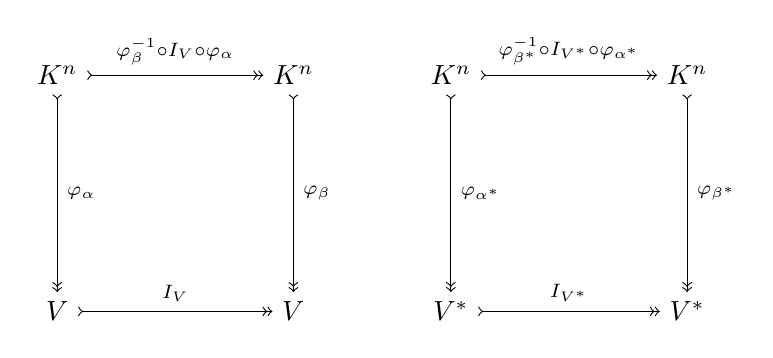
\begin{tikzpicture}[auto]
    \node (a) at (0, 3) {$K^n $};
    \node (b) at (0, 0) {$V$};
    \node (c) at (3, 3) {$K^n $};
    \node (d) at (3, 0) {$V$};
    \draw [>->>] (a) to node {$\scriptstyle \varphi_{\beta }^{-1} \circ I_V \circ \varphi_{\alpha } $} (c);
    \draw [>->>] (a) to node {$\scriptstyle \varphi_{\alpha } $} (b);
    \draw [>->>] (c) to node {$\scriptstyle \varphi_{\beta } $} (d);
    \draw [>->>] (b) to node {$\scriptstyle I_V $} (d);
    \node (a) at (5, 3) {$K^n $};
    \node (b) at (5, 0) {$V^* $};
    \node (c) at (8, 3) {$K^n $};
    \node (d) at (8, 0) {$V^* $};
    \draw [>->>] (a) to node {$\scriptstyle \varphi_{\beta^* }^{-1} \circ I_{V^* } \circ \varphi_{\alpha^* } $} (c);
    \draw [>->>] (a) to node {$\scriptstyle \varphi_{\alpha^* } $} (b);
    \draw [>->>] (c) to node {$\scriptstyle \varphi_{\beta^* } $} (d);
    \draw [>->>] (b) to node {$\scriptstyle I_{V^* } $} (d);
  \end{tikzpicture}
\end{center}
標準直交基底を$\left\langle \mathbf{e}_{i} \right\rangle_{i \in \varLambda_{n}}$とおいて$\forall j \in \varLambda_{n}$に対し、次のようになる。
\begin{align*}
\mathbf{w}_{j} &= I_{V}\left( \mathbf{w}_{j} \right)\\
&= \varphi_{\alpha} \circ \varphi_{\alpha}^{- 1} \circ I_{V}^{- 1} \circ \varphi_{\beta} \circ \varphi_{\beta}^{- 1}\left( \mathbf{w}_{j} \right)\\
&= \varphi_{\alpha} \circ \left( \varphi_{\beta}^{- 1} \circ I_{V} \circ \varphi_{\alpha} \right)^{- 1} \circ \varphi_{\beta}^{- 1}\left( \mathbf{w}_{j} \right)\\
&= \varphi_{\alpha} \circ \left( \varphi_{\beta}^{- 1} \circ I_{V} \circ \varphi_{\alpha} \right)^{- 1}\left( \mathbf{e}_{j} \right)\\
&= \varphi_{\alpha}\left( {\left[ I_{V} \right]^{\beta}_{\alpha}}^{- 1}\mathbf{e}_{j} \right)\\
&= \varphi_{\alpha}\begin{pmatrix}
p_{11} & \cdots & p_{1j} & \cdots & p_{1n} \\
 \vdots & \ddots & \vdots & \ddots & \vdots \\
p_{j1} & \cdots & p_{jj} & \cdots & p_{jn} \\
 \vdots & \ddots & \vdots & \ddots & \vdots \\
p_{n1} & \cdots & p_{nj} & \cdots & p_{nn} \\
\end{pmatrix}\begin{pmatrix}
0 \\
 \vdots \\
1 \\
 \vdots \\
0 \\
\end{pmatrix}\\
&= \varphi_{\alpha}\begin{pmatrix}
p_{1j} \\
p_{2j} \\
 \vdots \\
p_{nj} \\
\end{pmatrix}\\
&= \varphi_{\alpha}\left( \sum_{i \in \varLambda_{n}} {p_{ij}\mathbf{e}_{i}} \right)\\
&= \sum_{i \in \varLambda_{n}} {p_{ij}\varphi_{\alpha}\left( \mathbf{e}_{i} \right)}\\
&= \sum_{i \in \varLambda_{n}} {p_{ij}\mathbf{v}_{i}}
\end{align*}
同様にして、$\forall j \in \varLambda_{n}$に対し、次式が得られる。
\begin{align*}
\chi_{j} = \sum_{i \in \varLambda_{n}} {q_{ij}\phi_{i}}
\end{align*}\par
したがって、次のようになる。
\begin{align*}
I_{n} &= \left( \delta_{ij} \right)_{(i,j) \in \varLambda_{n}^{2}}\\
&= \left( D_{V}\left( \mathbf{w}_{i},\chi_{j} \right) \right)_{(i,j) \in \varLambda_{n}^{2}}\\
&= \left( D_{V}\left( \sum_{k \in \varLambda_{n}} {p_{ki}\mathbf{v}_{k}},\sum_{l \in \varLambda_{n}} {q_{lj}\phi_{l}} \right) \right)_{(i,j) \in \varLambda_{n}^{2}}\\
&= \left( \sum_{k \in \varLambda_{n}} {\sum_{l \in \varLambda_{n}} {p_{ki}q_{lj}D_{V}\left( \mathbf{v}_{k},\phi_{l} \right)}} \right)_{(i,j) \in \varLambda_{n}^{2}}\\
&= \left( \sum_{k \in \varLambda_{n}} {\sum_{l \in \varLambda_{n}} {p_{ki}q_{lj}\delta_{kl}}} \right)_{(i,j) \in \varLambda_{n}^{2}}\\
&= \left( \sum_{k \in \varLambda_{n}} {p_{ki}q_{kj}} \right)_{(i,j) \in \varLambda_{n}^{2}}\\
&= \begin{pmatrix}
p_{11} & p_{21} & \cdots & p_{n1} \\
p_{12} & p_{22} & \cdots & p_{n2} \\
 \vdots & \vdots & \ddots & \vdots \\
p_{1n} & p_{2n} & \cdots & p_{nn} \\
\end{pmatrix}\begin{pmatrix}
q_{11} & q_{12} & \cdots & q_{1n} \\
q_{21} & q_{22} & \cdots & q_{2n} \\
 \vdots & \vdots & \ddots & \vdots \\
q_{n1} & q_{n2} & \cdots & q_{nn} \\
\end{pmatrix}\\
&={}^{t}\begin{pmatrix}
p_{11} & p_{12} & \cdots & p_{1n} \\
p_{21} & p_{22} & \cdots & p_{2n} \\
 \vdots & \vdots & \ddots & \vdots \\
p_{n1} & p_{n2} & \cdots & p_{nn} \\
\end{pmatrix}\begin{pmatrix}
q_{11} & q_{12} & \cdots & q_{1n} \\
q_{21} & q_{22} & \cdots & q_{2n} \\
 \vdots & \vdots & \ddots & \vdots \\
q_{n1} & q_{n2} & \cdots & q_{nn} \\
\end{pmatrix}\\
&={}^{t}{\left[ I_{V} \right]^{\beta}_{\alpha}}^{- 1}{\left[ I_{V^{*}} \right]^{\beta^{*}}_{\alpha^{*}}}^{- 1}\\
&= \left( \left[ I_{V^{*}} \right]^{\beta^{*}}_{\alpha^{*}}{}^{t}\left[ I_{V} \right]^{\beta}_{\alpha} \right)^{- 1}
\end{align*}
よって、$\left[ I_{V^{*}} \right]^{\beta^{*}}_{\alpha^{*}}{}^{t}\left[ I_{V} \right]^{\beta}_{\alpha} = I_{n}$が得られる。
\end{proof}
\begin{thm}\label{2.4.3.14}
体$K$上の$n$次元vector空間$V$の双対空間$V^{*}$について、そのvector空間$V$の基底たち$\left\langle \mathbf{v}_{i} \right\rangle_{i \in \varLambda_{n}}$、$\left\langle \mathbf{w}_{i} \right\rangle_{i \in \varLambda_{n}}$、これらのその双対空間$V^{*}$の双対基底たち$\left\langle \phi_{i} \right\rangle_{i \in \varLambda_{n}}$、$\left\langle \chi_{i} \right\rangle_{i \in \varLambda_{n}}$が与えられたとき、これらを$\alpha = \left\langle \mathbf{v}_{i} \right\rangle_{i \in \varLambda_{n}}$、$\beta = \left\langle \mathbf{w}_{i} \right\rangle_{i \in \varLambda_{n}}$、$\alpha^{*} = \left\langle \phi_{i} \right\rangle_{i \in \varLambda_{n}}$、$\beta^{*} = \left\langle \chi_{i} \right\rangle_{i \in \varLambda_{n}}$とおかれると、次のことは同値である。
\begin{itemize}
\item
  それらの基底たち$\alpha$、$\beta$、$\alpha^{*}$、$\beta^{*}$の基底変換における線形同型写像がそれぞれ$\varphi_{\alpha}$、$\varphi_{\beta}$、$\varphi_{\alpha^{*}}$、$\varphi_{\beta^{*}}$とおかれると、$\varphi_{\alpha^{*}} \circ \varphi_{\alpha}^{- 1} = \varphi_{\beta^{*}} \circ \varphi_{\beta}^{- 1}$が成り立つ。
\item
  その基底$\alpha$からその基底$\beta$への基底変換行列$\left[ I_{V} \right]^{\beta}_{\alpha}$、その基底$\alpha^{*}$からその基底$\beta^{*}$への基底変換行列$\left[ I_{V^{*}} \right]^{\beta^{*}}_{\alpha^{*}}$について、$\left[ I_{V} \right]^{\beta}_{\alpha} ={}^{t}{\left[ I_{V} \right]^{\beta}_{\alpha}}^{- 1}$が成り立つ。
\item
  その基底$\alpha$からその基底$\beta$への基底変換行列$\left[ I_{V} \right]^{\beta}_{\alpha}$、その基底$\alpha^{*}$からその基底$\beta^{*}$への基底変換行列$\left[ I_{V^{*}} \right]^{\beta^{*}}_{\alpha^{*}}$について、$\left[ I_{V^{*}} \right]^{\beta^{*}}_{\alpha^{*}} ={}^{t}{\left[ I_{V^{*}} \right]^{\beta^{*}}_{\alpha^{*}}}^{- 1}$が成り立つ。
\end{itemize}
\end{thm}
\begin{proof}
体$K$上の$n$次元vector空間$V$の双対空間$V^{*}$について、そのvector空間$V$の基底たち$\left\langle \mathbf{v}_{i} \right\rangle_{i \in \varLambda_{n}}$、$\left\langle \mathbf{w}_{i} \right\rangle_{i \in \varLambda_{n}}$、これらのその双対空間$V^{*}$の双対基底たち$\left\langle \phi_{i} \right\rangle_{i \in \varLambda_{n}}$、$\left\langle \chi_{i} \right\rangle_{i \in \varLambda_{n}}$が与えられたとき、これらを$\alpha = \left\langle \mathbf{v}_{i} \right\rangle_{i \in \varLambda_{n}}$、$\beta = \left\langle \mathbf{w}_{i} \right\rangle_{i \in \varLambda_{n}}$、$\alpha^{*} = \left\langle \phi_{i} \right\rangle_{i \in \varLambda_{n}}$、$\beta^{*} = \left\langle \chi_{i} \right\rangle_{i \in \varLambda_{n}}$、それらの基底たち$\alpha$、$\beta$、$\alpha^{*}$、$\beta^{*}$の基底変換における線形同型写像がそれぞれ$\varphi_{\alpha}$、$\varphi_{\beta}$、$\varphi_{\alpha^{*}}$、$\varphi_{\beta^{*}}$とおかれると、次式が成り立つことから、
\begin{center}
  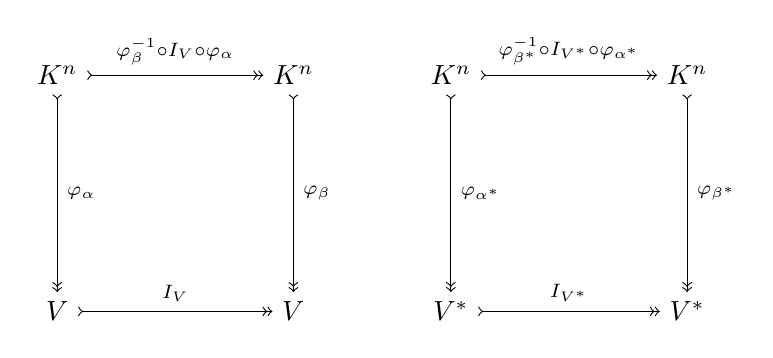
\begin{tikzpicture}[auto]
    \node (a) at (0, 3) {$K^n $};
    \node (b) at (0, 0) {$V$};
    \node (c) at (3, 3) {$K^n $};
    \node (d) at (3, 0) {$V$};
    \draw [>->>] (a) to node {$\scriptstyle \varphi_{\beta }^{-1} \circ I_V \circ \varphi_{\alpha } $} (c);
    \draw [>->>] (a) to node {$\scriptstyle \varphi_{\alpha } $} (b);
    \draw [>->>] (c) to node {$\scriptstyle \varphi_{\beta } $} (d);
    \draw [>->>] (b) to node {$\scriptstyle I_V $} (d);
    \node (a) at (5, 3) {$K^n $};
    \node (b) at (5, 0) {$V^* $};
    \node (c) at (8, 3) {$K^n $};
    \node (d) at (8, 0) {$V^* $};
    \draw [>->>] (a) to node {$\scriptstyle \varphi_{\beta^* }^{-1} \circ I_{V^* } \circ \varphi_{\alpha^* } $} (c);
    \draw [>->>] (a) to node {$\scriptstyle \varphi_{\alpha^* } $} (b);
    \draw [>->>] (c) to node {$\scriptstyle \varphi_{\beta^* } $} (d);
    \draw [>->>] (b) to node {$\scriptstyle I_{V^* } $} (d);
  \end{tikzpicture}
\end{center}
次式が得られる。
\begin{center}
  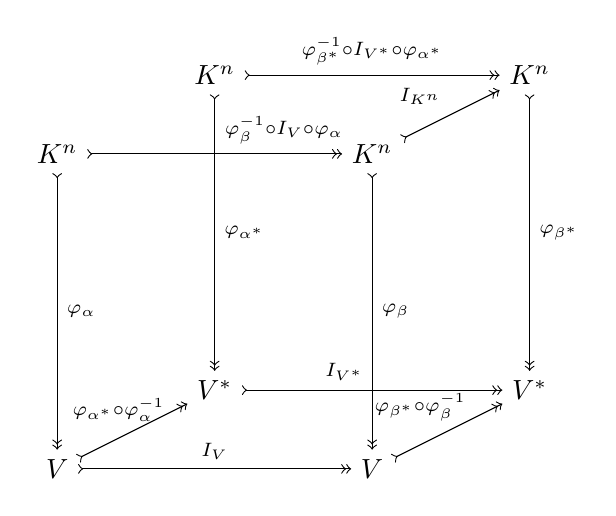
\begin{tikzpicture}[auto]
    \node (a) at (0, 4) {$K^n $};
    \node (b) at (0, 0) {$V$};
    \node (c) at (4, 4) {$K^n $};
    \node (d) at (4, 0) {$V$};
    \node (e) at (2, 5) {$K^n $};
    \node (f) at (2, 1) {$V^* $};
    \node (g) at (6, 5) {$K^n $};
    \node (h) at (6, 1) {$V^* $};
    \draw [>->>] (a) to node[xshift=25pt, yshift=0pt] {$\scriptstyle \varphi_{\beta }^{-1} \circ I_V \circ \varphi_{\alpha } $} (c);
    \draw [>->>] (a) to node {$\scriptstyle \varphi_{\alpha } $} (b);
    \draw [>->>] (c) to node {$\scriptstyle \varphi_{\beta } $} (d);
    \draw [>->>] (b) to node {$\scriptstyle I_V $} (d);
    \draw [>->>] (e) to node {$\scriptstyle \varphi_{\beta^* }^{-1} \circ I_{V^* } \circ \varphi_{\alpha^* } $} (g);
    \draw [>->>] (e) to node {$\scriptstyle \varphi_{\alpha^* } $} (f);
    \draw [>->>] (g) to node {$\scriptstyle \varphi_{\beta^* } $} (h);
    \draw [>->>] (f) to node[xshift=-10pt, yshift=0pt] {$\scriptstyle I_{V^* } $} (h);
    \draw [>->>] (b) to node[xshift=15pt, yshift=0pt] {$\scriptstyle \varphi_{\alpha^* } \circ \varphi_{\alpha }^{-1} $} (f);
    \draw [>->>] (d) to node[xshift=10pt, yshift=0pt] {$\scriptstyle \varphi_{\beta^* } \circ \varphi_{\beta }^{-1} $} (h);
    \draw [>->>] (c) to node {$\scriptstyle I_{K^n } $} (g);
    \end{tikzpicture}
\end{center}
これにより、次式のようになる\footnote{愚直に計算するなら、次のようになる。
\begin{align*}
\varphi_{\beta^{*}} \circ \varphi_{\beta}^{- 1} &= \varphi_{\alpha^{*}} \circ \varphi_{\alpha^{*}}^{- 1} \circ \varphi_{\beta^{*}}^{- 1} \circ \varphi_{\beta} \circ \varphi_{\alpha} \circ \varphi_{\alpha}^{- 1} \\
&= I_{V^{*}} \circ \varphi_{\alpha^{*}} \circ \varphi_{\alpha^{*}}^{- 1} \circ I_{V^{*}}^{- 1} \circ \varphi_{\beta^{*}} \circ I_{K^{n}} \circ \varphi_{\beta}^{- 1} \circ I_{V} \circ \varphi_{\alpha} \circ \varphi_{\alpha}^{- 1} \circ I_{V}^{- 1} \\
&= I_{V^{*}} \circ \varphi_{\alpha^{*}} \circ \left( \varphi_{\beta^{*}}^{- 1} \circ I_{V^{*}} \circ \varphi_{\alpha^{*}} \right)^{- 1} \circ I_{K^{n}} \circ \left( \varphi_{\beta}^{- 1} \circ I_{V} \circ \varphi_{\alpha} \right) \circ \varphi_{\alpha}^{- 1} \circ I_{V}^{- 1}
\end{align*}}。
\begin{align*}
\varphi_{\beta^{*}} \circ \varphi_{\beta}^{- 1} &= I_{V^{*}} \circ \varphi_{\alpha^{*}} \circ \left( \varphi_{\beta^{*}}^{- 1} \circ I_{V^{*}} \circ \varphi_{\alpha^{*}} \right)^{- 1} \circ I_{K^{n}} \circ \left( \varphi_{\beta}^{- 1} \circ I_{V} \circ \varphi_{\alpha} \right) \circ \varphi_{\alpha}^{- 1} \circ I_{V}^{- 1}\\
&= \varphi_{\alpha^{*}} \circ \left( \varphi_{\beta^{*}}^{- 1} \circ I_{V^{*}} \circ \varphi_{\alpha^{*}} \right)^{- 1} \circ \left( \varphi_{\beta}^{- 1} \circ I_{V} \circ \varphi_{\alpha} \right) \circ \varphi_{\alpha}^{- 1}
\end{align*}\par
したがって、$\varphi_{\alpha^{*}} \circ \varphi_{\alpha}^{- 1} = \varphi_{\beta^{*}} \circ \varphi_{\beta}^{- 1}$が成り立つなら、上記の議論により次のようになる。
\begin{align*}
\varphi_{\beta}^{- 1} \circ I_{V} \circ \varphi_{\alpha} &= \left( \varphi_{\beta^{*}}^{- 1} \circ I_{V^{*}} \circ \varphi_{\alpha^{*}} \right) \circ \left( \varphi_{\beta^{*}}^{- 1} \circ I_{V^{*}} \circ \varphi_{\alpha^{*}} \right)^{- 1} \circ \left( \varphi_{\beta}^{- 1} \circ I_{V} \circ \varphi_{\alpha} \right)\\
&= \left( \varphi_{\beta^{*}}^{- 1} \circ I_{V^{*}} \circ \varphi_{\alpha^{*}} \right) \circ \left( \varphi_{\beta^{*}}^{- 1} \circ I_{V^{*}} \circ \varphi_{\alpha^{*}} \right)^{- 1} \circ \left( \varphi_{\beta}^{- 1} \circ I_{V} \circ \varphi_{\alpha} \right)\\
&= \left( \varphi_{\beta^{*}}^{- 1} \circ I_{V^{*}} \circ \varphi_{\alpha^{*}} \right) \circ \varphi_{\alpha^{*}}^{- 1} \circ \varphi_{\alpha^{*}} \circ \left( \varphi_{\beta^{*}}^{- 1} \circ I_{V^{*}} \circ \varphi_{\alpha^{*}} \right)^{- 1} \\
&\quad \circ \left( \varphi_{\beta}^{- 1} \circ I_{V} \circ \varphi_{\alpha} \right) \circ \varphi_{\alpha}^{- 1} \circ \varphi_{\alpha}\\
&= \left( \varphi_{\beta^{*}}^{- 1} \circ I_{V^{*}} \circ \varphi_{\alpha^{*}} \right) \circ \varphi_{\alpha^{*}}^{- 1} \circ \varphi_{\beta^{*}} \circ \varphi_{\beta}^{- 1} \circ \varphi_{\alpha}\\
&= \left( \varphi_{\beta^{*}}^{- 1} \circ I_{V^{*}} \circ \varphi_{\alpha^{*}} \right) \circ \varphi_{\alpha^{*}}^{- 1} \circ \varphi_{\alpha^{*}} \circ \varphi_{\alpha}^{- 1} \circ \varphi_{\alpha}\\
&= \varphi_{\beta^{*}}^{- 1} \circ I_{V^{*}} \circ \varphi_{\alpha^{*}}
\end{align*}
ゆえに、$\left[ I_{V} \right]^{\beta}_{\alpha} = \left[ I_{V^{*}} \right]^{\beta^{*}}_{\alpha^{*}}$が得られる。その写像$\varphi_{\beta^{*}}^{- 1} \circ I_{V^{*}} \circ \varphi_{\alpha^{*}}$が線形同型写像であることに注意すれば、定理\ref{2.4.3.13}より$\left[ I_{V^{*}} \right]^{\beta^{*}}_{\alpha^{*}} ={}^{t}{\left[ I_{V} \right]^{\beta}_{\alpha}}^{- 1}$が成り立つので、$\left[ I_{V} \right]^{\beta}_{\alpha} ={}^{t}{\left[ I_{V} \right]^{\beta}_{\alpha}}^{- 1}$が成り立つ。\par
逆に、$\left[ I_{V} \right]^{\beta}_{\alpha} ={}^{t}{\left[ I_{V} \right]^{\beta}_{\alpha}}^{- 1}$が成り立つなら、その写像$\varphi_{\beta^{*}}^{- 1} \circ I_{V^{*}} \circ \varphi_{\alpha^{*}}$が線形同型写像であることに注意すれば、定理\ref{2.4.3.13}より$\left[ I_{V^{*}} \right]^{\beta^{*}}_{\alpha^{*}} ={}^{t}{\left[ I_{V} \right]^{\beta}_{\alpha}}^{- 1} = \left[ I_{V} \right]^{\beta}_{\alpha}$が成り立つので、$\varphi_{\beta}^{- 1} \circ I_{V} \circ \varphi_{\alpha} = \varphi_{\beta^{*}}^{- 1} \circ I_{V^{*}} \circ \varphi_{\alpha^{*}}$が成り立つことにより次のようになる。
\begin{align*}
\varphi_{\alpha^{*}} \circ \varphi_{\alpha}^{- 1} &= \varphi_{\alpha^{*}} \circ \left( \varphi_{\beta}^{- 1} \circ I_{V} \circ \varphi_{\alpha} \right)^{- 1} \circ \left( \varphi_{\beta}^{- 1} \circ I_{V} \circ \varphi_{\alpha} \right) \circ \varphi_{\alpha}^{- 1}\\
&= \varphi_{\alpha^{*}} \circ \left( \varphi_{\beta^{*}}^{- 1} \circ I_{V^{*}} \circ \varphi_{\alpha^{*}} \right)^{- 1} \circ \left( \varphi_{\beta}^{- 1} \circ I_{V} \circ \varphi_{\alpha} \right) \circ \varphi_{\alpha}^{- 1}\\
&= \varphi_{\alpha^{*}} \circ \varphi_{\alpha^{*}}^{- 1} \circ I_{V^{*}}^{- 1} \circ \varphi_{\beta^{*}} \circ \varphi_{\beta}^{- 1} \circ I_{V} \circ \varphi_{\alpha} \circ \varphi_{\alpha}^{- 1}\\
&= \varphi_{\beta^{*}} \circ \varphi_{\beta}^{- 1}
\end{align*}\par
$\left[ I_{V^{*}} \right]^{\beta^{*}}_{\alpha^{*}} ={}^{t}{\left[ I_{V^{*}} \right]^{\beta^{*}}_{\alpha^{*}}}^{- 1}$が成り立つことについても同様にして示される。
\end{proof}
\begin{thebibliography}{50}
  \bibitem{1}
  松坂和夫, "線型代数入門", 岩波書店, 1980. 新装版第2刷 p319-333 ISBN978-4-00-029872-8
  \bibitem{2}
  佐武一郎, 線型代数学, 裳華房, 1958. 第53版 p193-197,200-202 ISBN4-7853-1301-3
\end{thebibliography}
\end{document}
